\documentclass[12t,letterpaper]{article}

\newenvironment{proof}{\noindent{\bf Proof:}}{\qed\bigskip}

\newtheorem{theorem}{Theorem}
\newtheorem{corollary}{Corollary}
\newtheorem{lemma}{Lemma} 
\newtheorem{claim}{Claim}
\newtheorem{fact}{Fact}
\newtheorem{definition}{Definition}
\newtheorem{assumption}{Assumption}
\newtheorem{observation}{Observation}
\newtheorem{example}{Example}
\newcommand{\qed}{\rule{7pt}{7pt}}

\newcommand{\assignment}[4]{
\thispagestyle{plain} 
\newpage
\setcounter{page}{1}
\noindent
\begin{center}
\framebox{ \vbox{ \hbox to 6.28in
{\bf CS446: Machine Learning \hfill #1}
\vspace{4mm}
\hbox to 6.28in
{\hspace{2.5in}\large\mbox{#2}}
\vspace{4mm}
\hbox to 6.28in
{{\it Handed Out: #3 \hfill Due: #4}}
}}
\end{center}
}

\newcommand{\solution}[3]{
\thispagestyle{plain} 
\newpage
\setcounter{page}{1}
\noindent
\begin{center}
\framebox{ \vbox{ \hbox to 6.28in
{\bf CS 374 \hfill #3}
\vspace{4mm}
\hbox to 6.28in
{\hspace{2.5in}\large\mbox{#2}}
\vspace{4mm}
\hbox to 6.28in
{#1 \hfill}
}}
\end{center}
\markright{#1}
}

\newenvironment{algorithm}
{\begin{center}
\begin{tabular}{|l|}
\hline
\begin{minipage}{1in}
\begin{tabbing}
\quad\=\qquad\=\qquad\=\qquad\=\qquad\=\qquad\=\qquad\=\kill}
{\end{tabbing}
\end{minipage} \\
\hline
\end{tabular}
\end{center}}

\def\Comment#1{\textsf{\textsl{$\langle\!\langle$#1\/$\rangle\!\rangle$}}}


\usepackage{amsmath, verbatim, tikz, float}

\usetikzlibrary{arrows,automata}

\oddsidemargin 0in
\evensidemargin 0in
\textwidth 6.5in
\topmargin -0.5in
\textheight 9.0in
\newcommand{\norm}[1]{\left\lVert #1 \right\rVert}
\begin{document}

\solution{Nikhil Unni (nunni2)}{Homework 2}{Spring 2015}
\pagestyle{myheadings}

\begin{enumerate}
\item
  \begin{enumerate}
  \item Draw an NFA that accepts the language {w | there is exactly one block of 0s of even length}.
    (A “block of 0s” is a substring of 0s that is not contained in any longer substring of 0s.)
    \begin{figure}[H]
    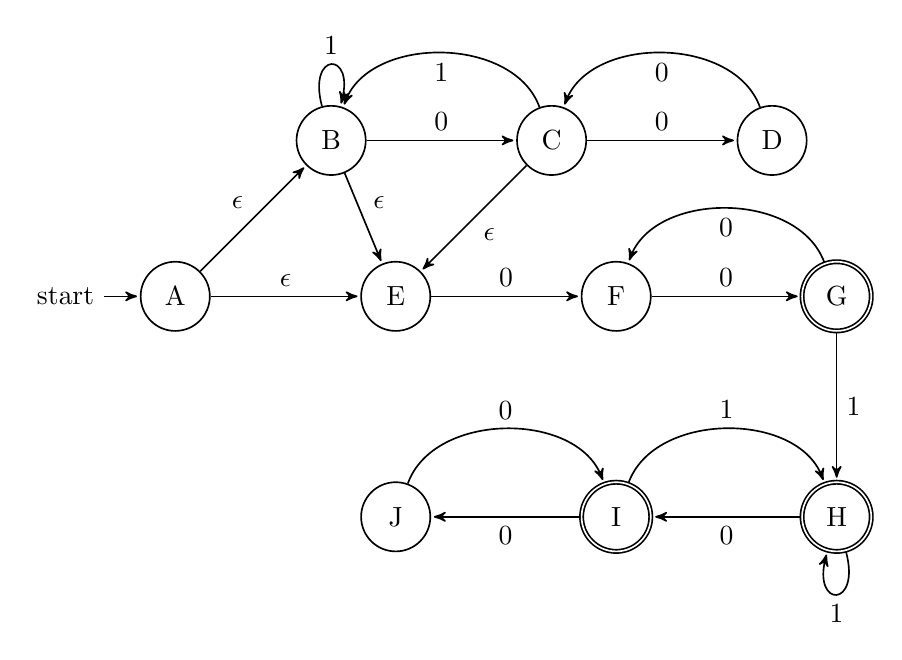
\begin{tikzpicture}[->,>=stealth',shorten >=1pt,auto,node distance=2.8cm, semithick]
      \tikzstyle{every state}=[fill=none,draw=black,text=black]
      
      \node[initial,state]   (A)                    {A};
      \node[state]           (B) [above right of=A] {B};
      \node[state]           (C) [right of=B]       {C};
      \node[state]           (D) [right of=C]       {D};
      
      \node[state]           (E) [right of=A]       {E};
      \node[state]           (F) [right of=E]       {F};
      \node[state,accepting] (G) [right of=F]       {G};
      
      \node[state,accepting] (H) [below of=G]       {H};
      \node[state,accepting] (I) [left of=H]        {I};
      \node[state]           (J) [left of=I]        {J};
      
      \path (A) edge                 node {$\epsilon$} (B)
                edge                 node {$\epsilon$} (E)
            (B) edge [loop above]    node {1}          (B)
                edge                 node {0}          (C)
                edge                 node {$\epsilon$} (E)
            (C) edge                 node {0}          (D)
                edge [bend right=70] node {1}          (B)
                edge                 node {$\epsilon$} (E)
            (D) edge [bend right=70] node {0}          (C)
            (E) edge                 node {0}          (F)
            (F) edge                 node {0}          (G)
            (G) edge [bend right=70] node {0}          (F)
                edge                 node {1}          (H)
            (H) edge [loop below]    node {1}          (H)
                edge                 node {0}          (I)
            (I) edge                 node {0}          (J)
                edge [bend left=70]  node {1}          (H)
            (J) edge [bend left=70]  node {0}          (I);            
    \end{tikzpicture}
    \end{figure}
  \item
    \begin{enumerate}
    \item Draw an NFA for the regular expression $(010)^{\text{*}} + (01)^{\text{*}} + 0^{\text{*}}$
      \begin{figure}[H]
      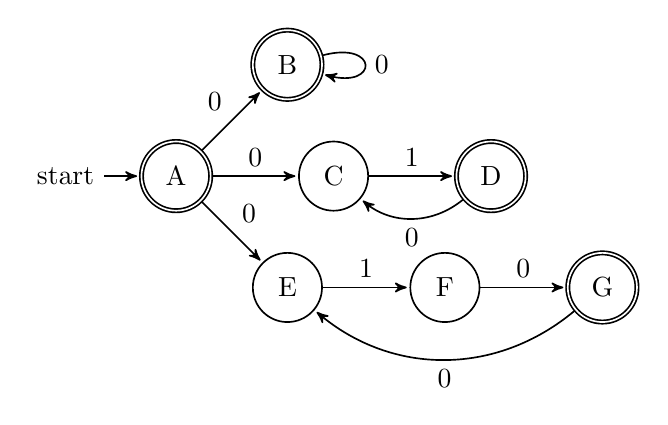
\begin{tikzpicture}[->,>=stealth',shorten >=1pt,auto,node distance=2.0cm, semithick]
        \tikzstyle{every state}=[fill=none,draw=black,text=black]
        \node[initial,state,accepting] (A)                    {A};

        \node[state,accepting]         (B) [above right of=A] {B};

        \node[state]                   (C) [right of=A]       {C};
        \node[state,accepting]         (D) [right of=C]       {D};

        \node[state]                   (E) [below right of=A] {E};
        \node[state]                   (F) [right of=E]       {F};
        \node[state,accepting]         (G) [right of=F]       {G};

        \path (A) edge                node {0} (B)
                  edge                node {0} (C)
                  edge                node {0} (E)
              (B) edge [loop right]   node {0} (B)
              (C) edge                node {1} (D)
              (D) edge [bend left=40] node {0} (C)
              (E) edge                node {1} (F)
              (F) edge                node {0} (G)
              (G) edge [bend left=40] node {0} (E);
      \end{tikzpicture}
      \end{figure}
    \item Now using the powerset construction (also called the subset construcion), design a DFA
      for the same language. Label the states of your DFA with names that are sets of states of
      your NFA.
      \begin{figure}[H]
      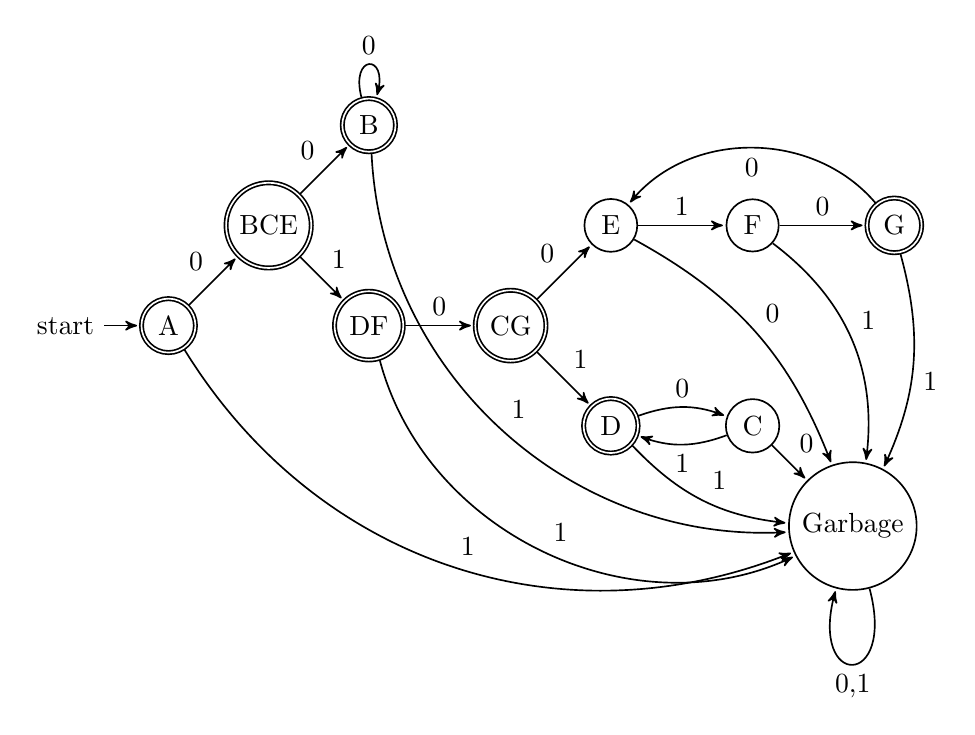
\begin{tikzpicture}[->,>=stealth',shorten >=1pt,auto,node distance=1.8cm, semithick]
        \tikzstyle{every state}=[fill=none,draw=black,text=black,minimum size=0pt]
        \node[initial,state,accepting] (A)                        {A};
        \node[state,accepting]         (BCE)     [above right of=A]   {BCE};
        \node[state,accepting]         (B)       [above right of=BCE] {B};
        \node[state,accepting]         (DF)      [below right of=BCE] {DF};
        \node[state,accepting]         (CG)      [right of=DF]        {CG};
        \node[state]                   (E)       [above right of=CG]  {E};
        \node[state,accepting]         (D)       [below right of=CG]  {D};
        \node[state]                   (F)       [right of=E]         {F};
        \node[state]                   (C)       [right of=D]         {C};
        \node[state,accepting]         (G)       [right of=F]         {G};
        \node[state]                   (Garbage) [below right of=C]   {Garbage};

        \path (A)   edge                 node {0} (BCE)
                    edge [bend right=40] node {1} (Garbage)
              (BCE) edge                 node {0} (B)
                    edge                 node {1} (DF)
              (B)   edge [loop above]    node {0} (B)
                    edge [bend right=45] node {1} (Garbage)
              (DF)  edge                 node {0} (CG)
                    edge [bend right=50] node {1} (Garbage)
              (CG)  edge                 node {0} (E)
                    edge                 node {1} (D)
              (E)   edge [bend left=20]  node {0} (Garbage)
                    edge                 node {1} (F)
              (D)   edge [bend left=20]  node {0} (C)
                    edge [bend right=20] node {1} (Garbage)
              (F)   edge                 node {0} (G)
                    edge [bend left=30]  node {1} (Garbage)
              (C)   edge                 node {0} (Garbage)
                    edge [bend left=20]  node {1} (D)
              (G)   edge [bend right=50] node {0} (E)
                    edge [bend left=20]  node {1} (Garbage)


              (Garbage) edge [loop below] node {0,1} (Garbage);
      \end{tikzpicture}
      \end{figure}
    \end{enumerate}
  \end{enumerate}
\end{enumerate}
\end{document}